% first example chapter
% @author Jan Robert Rösler 
%
\chapter{Neuronale Navigation mit Bilddaten}

\section{Relevante Technik/Hintergrund}
Hier soll zunächst eine kurze Beschreibung der für Neuronale Navigation auf Bilddaten relevanten Technik erfolgen. Grundlegendes wird nur der Vollständigkeit halber erwähnt, speziellere Aspekte kurz vorgestellt. 

CNN 

RESIDUAL (BLOCK)

LAYER FREEZING 

PreProcessing (?)



\section{Ansätze}
\note{Hier werden Paper vorgestellt, die Geschichte der Navigation auf Bilddaten und wie das fumktiojneiren kann --> Ansätze}

Versuche durch neuronale Verarbeitung von reinen Bilddaten in einem Szenario zu navigieren, gabe es bereits 1989 \cite{pomerleau1989alvinn}.
Das Netzwerk ALVINN (Autonomous Land Vehicle In a Neural Network) sollte das NAVLAB steuern, ein Testfahrzeug für Autonome Navigation der Carnegie Mellon University.
In \ref{img:ALVINNa} lässt sich die Architektur nachvollziehen. 
Der rein visuelle Input (die Blautstufenintensität eines Pixels bestimmt das Aktivierungslevel des Inputneurons) wird untersützt durch eine laserbasierte Abstandsmessung und ein Inputneuron für die Kodierung der \glqq Straßenintensität\grqq{}, also ob die Straße heller oder dunkler wird.
Aus heutiger Sicht ist das Netz mit nur einer hidden Layer mit 29 Neronen sehr klein, die im weiteren angesprochenen Architekturen haben bis zu 50 Layer mit 26 Million Parametern. 
Zudem interpretiert ALVINN die Aufgabe des Spurfolgens nicht als Regressionsproblem, sondern als Klassifikation. Die Ausgangsneuronen sind eine lineare Repräsentation der Lenkrichtung, die das Fahrzeug in Richtung Fahrbahnmitte steuert. Neuronen in der Mitte stehen für eine Fahrt geradeaus, Neuronen links und rechts für die jeweilige Fahrtrichtung.
Grob gesagt gibt das Neuron mit dem höchsten Aktivierungslevel die Fahrtrichtung (den einzuschlagenden Lenkwinkel) an.
Im Ergebnis konnte das Netz nach 40 Epochen Training auf simulierten Fahrbahnbildern, zu sehen in \ref{img:ALVINNb}, einen 400 Meter Weg durch einen Wald mit \SI{1/2}{\meter/\second} sicher abfahren



\begin{figure}
	\centering
	\begin{subfigure}{.5\textwidth}
	\centering
		  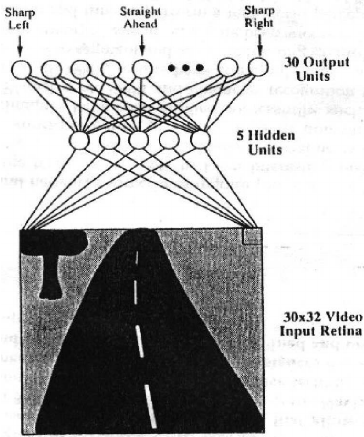
\includegraphics[width=.85\linewidth]{figures/Architecture-ALVINN.png}
		  \caption{}
		  \label{img:ALVINNa}
	\end{subfigure}%
	\begin{subfigure}{.5\textwidth}
	\centering
		  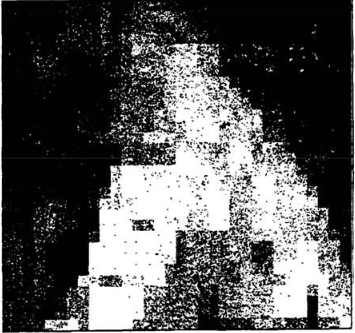
\includegraphics[width=.85\linewidth]{figures/Strasse-ALVINN.png}
	 	  \caption{}
		  \label{img:ALVINNb}
	\end{subfigure}%
	\caption{ALVINN Architektur (a) und simulierte Fahrbahn (b)}
	%Quelle: \protect\citeI{Architecture-ALVINN}
	\label{img:ALVINN}
\end{figure}



 Präsentation ALVINN, dann gegenüberstellung mit modernem Netzwerk a la NVIDIA.






Kurzer Blick auf  Self driving car steering angle4 prediction und berkeley (large scale video sets) (vielleicht auchSPÄTER)







